% !TEX root =  manuscript.tex
\subsection{Rationale (RQ2)}

The goal of this RQ is to understand the \textit{motivations}
behind the use of visual approaches in the collected publications.
\changed{For each paper in our pool, we analyzed the paper's full text and 
noted down the rationales mentioned by the authors for using computer vision to solve the software engineering problem being tackled.
This resulted in three main categories, namely, \textit{context-driven, ease of use,} and \textit{robustness} (as will be described below). For each paper that did not explicitly mention their rationale, we analyzed the text and classified the paper to the closest rationale category. We now describe the three identified categories of rationale.}

\header{Context-driven} 
Computer vision has been utilized
because the context is intrinsically \textit{visual} in nature,
which is the case in all the papers that focused on GUIs.
Thus, it was natural for the authors to deal with a visual artifact through a computer vision technique.
More than half of the selected papers motivate the use of visual approaches
as such~\cite{Burg-2015-UIST,Feng-2016-ASE,Deka-2016-UIST,Deka-2017-UIST,canvas_icst2018,
Patric-2016-ASE,Wan-2017-STVR,Scharf-2013-ICSE,Ponzanelli-2016-ICSE,Reiss-2018-ASEj,
Bao-2017-EMSE,Nguyen-2015-ASE,Kirac-2018-JSS,Leotta-2018-STVR,Li-2010-CHI,
Amalfitano-2014-WISE,Selay-2014-DICTA,Mahajan-2015-ICST,Mahajan-2016-ICST,
He-2016-ICWS,Chen-2017-IUI,Xu-2018-TOIT,Delamaro-2011-STVR,Kuchta-2018-EMSE,
Chang-2010-CHI,Alegroth-2013-ICST}. 

For instance, \citet{Chang-2010-CHI} describe two properties of visual approaches
that make them particularly appealing for analyzing GUI-based software:
\textit{intuitiveness} and \textit{universality}.
They describe how for certain tasks, using visual artifacts---such as a GUI screenshot---
is a more spontaneous way of interaction with the software.
Due to their graphical nature, elements on the GUI can be most directly represented
by screenshots. Non-visual alternatives, such as scripting, would instead require users
to manipulate GUI elements through keywords which is arguably less intuitive. 

Furthermore, screenshots are easily accessible for all GUI-based applications.
Indeed, it is virtually always possible to take a screenshot of a GUI element,
across all applications and platforms. This can make it attractive to propose techniques 
based on analyzing visual artifacts.

\header{Ease of Use}
As a second main motivation, researchers have utilized visual approaches
because they deemed them \emph{easier} to use by end users~\cite{Choudhary-2012-ICST,
Semenenko-2013-ICSM,Choudhary-2013-ICSE,Mahajan-2014-ASE,Zhang-2017-ASE,
Choudhary-2010-ICSM,Lin-2014-TSE,Amalfitano-2014-WISE,Selay-2014-DICTA,
Mahajan-2015-ICST,Mahajan-2016-ICST,He-2016-ICWS,Chen-2017-IUI,
Xu-2018-TOIT,Delamaro-2011-STVR,Kuchta-2018-EMSE}. 
%
For instance, \citet{Zhang-2017-ASE} propose a tool that allows developers
to draw (e.g. via tablets, digital pens) simple sketches on app screenshots.
The tool then uses CV algorithms to analyze the shapes and structure of these hand
drawn sketches to decode the meaning of each sketch.
The tool then uses the sketch as a visual test spec to automatically
generate a number of GUI test suites for mobile applications.
The authors argue, and demonstrate, that providing developers with the option
of using simple hand sketches to automatically generate test cases
is a more natural and easier to use approach to create test cases compared to manually writing the test cases.


\begin{figure}
    \revised{\linewidth}{
\centering
%\fbox{
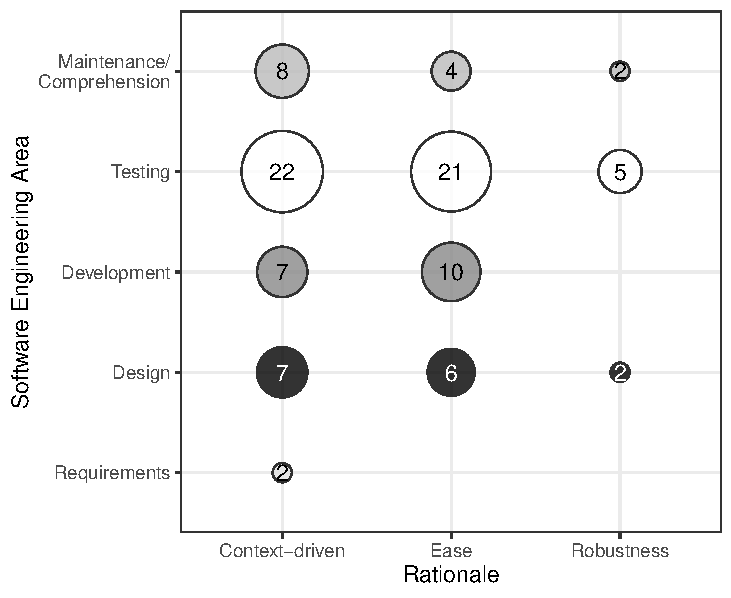
\includegraphics[width=0.8\linewidth]{survey/figures/bubbleplot-rq2.pdf}
%}
\caption{Distribution of rationales per SE area.}\label{fig:bubbleplot-rq2}
    }
\end{figure}

This viewpoint is also evident in papers targeting the detection of cross-browser
incompatibilities (XBIs)~\cite{Choudhary-2010-ICSM, Choudhary-2012-ICST, Semenenko-2013-ICSM,
Choudhary-2013-ICSE, Selay-2014-DICTA, He-2016-ICWS, Xu-2018-TOIT}.
This problem requires developers to detect visual differences between web pages within the same web application when rendered on different browsers.
This task is challenging for a number of reasons. 
First, manually performing this task, for instance through eyeballing, is neither efficient nor easy.
Hence, an automatic technique would require simulating
the reasoning that humans do while \textit{seeing and comparing} two web pages.
This can be easily simulated through a computer vision technique called \textit{image differencing}, for which a plethora of different techniques have been proposed~\cite{Choudhary-2012-ICST,
	Semenenko-2013-ICSM,Choudhary-2013-ICSE}.

However, originally, the same problem was tackled from a non-visual perspective.
First works on XBIs used well-known DOM differencing techniques as a proxy for finding visual defects. %~\cite{}. \andrea{pending cite}
The main limitation was the fact that DOM-level differences do not always
correspond to a different visual layout.
Hence, this caused such techniques to have many false positives and a low accuracy.
On the other hand, visual approaches have been proposed both as an alternative,
as well as, a complementary technique to overcome the limitations of the DOM-based approaches. 

\header{Robustness}
The concept of robustness of a visual approach concerns its capability of maintaining
its effectiveness despite minor visual changes happening in the software being analyzed.

A few papers~\cite{Chang-2010-CHI,Alegroth-2013-ICST,Tanno-2018-ICSTW} mention robustness
as rationale for choosing computer vision.
They explain that visual approaches are used because they are considered more change-tolerant than
alternative code-based techniques. In other words, according to the authors, using a code-based approach for the
same problem is likely to produce a fragile tool that would require a high maintenance cost. 

For instance, \citet{Chang-2010-CHI} describe how spatial re-arrangements of GUI components on the page
can lead to fragile test scripts, a well-known issue in web testing~\cite{Leotta-2016-JSEP}.
According to \citet{Chang-2010-CHI}, visual approaches are more robust to minor layout changes and
elements repositioning.
This viewpoint is discussed and confirmed in the paper by \citet{Alegroth-2013-ICST},
in which image recognition of GUI elements allows the development of more robust system-level automated test suites. 
A similar finding is in the paper by \citet{Stocco-2018-FSE}, in which an image processing pipeline was used to automatically trace web elements across different versions of the same web applications. Their tool \textsc{Vista} exhibited a high test repair rate during software evolution, outperforming a DOM-based test repair solution. This essentially means that in the web domain, web app GUIs exhibit less frequent changes as compared to the DOM, as acknowledged by other researchers~\cite{2015-Leotta-ICST,2016-Leotta-JSEP,Hammoudi-2016-FSE,Hammoudi-2016-ICST}.

The bubble chart of \Cref{fig:bubbleplot-rq2} shows the distribution of the rationales
in relation to the SE areas presented in \Cref{sec:rq1}.
We notice that the context-driven category dominates across all SE areas.
In the areas of requirements, design, and maintenance, visual approaches were
prevalently used because, at this stage of the software development lifecycle,
designers or requirements engineers mostly deal with visual abstractions of
(portions) the software such as GUI mockups, or UML models.
Computer vision allows the transformation of these visual artifacts to support successive SE tasks.
For example, in the work by~\citet{Zhang-2017-ASE}, annotated sketches are used
to specify test requirements and test case creation. In this case, the targeted SE
area is both requirements engineering and testing. 


\header{Summary}
In this section, 
the goal was to understand the rationales and motivations for using computer vision to
address software engineering problems.
An understanding of the rationales can help researchers
decide if their research area or topic has similar problems or challenges,
and then potentially explore using computer vision for their problem.
We identified three types of rationales by collecting and categorizing the reasons stated by the authors of each paper. There are context-driven, ease of use, and robustness.
Papers were classified as context-driven when the context of the software engineering problem itself
has dictated the use of visual approaches.
The ease of use classification was used in cases where the motivation
is not necessarily driven by the context,
but driven by the motivation of making an existing software engineering process easier to use
(e.g. has less manual work, easier to comprehend).
Finally, papers were classified as motivated by robustness whenever the motivation
is making a software engineering task more accurate or less fragile.
Out of all three categories of rationales, the context-driven category was the most common.





